\documentclass[10pt,letterpaper]{article}
\usepackage[margin=.7in]{geometry}
\usepackage{graphicx,amsmath,fontspec,unicode-math}
\setmainfont{NimbusRoman-Regular.otf}
\setsansfont{NimbusSans-Regular.otf}
\setmathfont{Latin Modern Math}
\setmainfont{Noto Serif CJK SC}
\XeTeXlinebreaklocale "zh"
\XeTeXlinebreakskip=0pt plus 1pt
\usepackage[hidelinks]{hyperref}
\hypersetup{pdfauthor={},pdftitle={机制补充图}}
\graphicspath{{../figures/}}
\pagestyle{plain}
\begin{document}
\section*{机制补充图 S1: 低频子空间选取}
本补充给出子空间选取、区域配额与gate生命周期的详细流程，适用条件与主文一致。\par\medskip
\noindent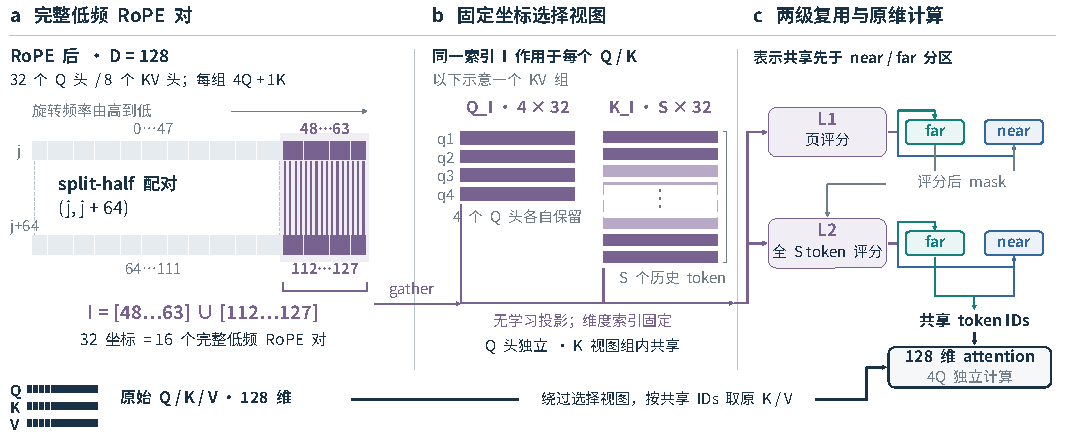
\includegraphics[width=\textwidth]{ppt_subspace_zh.pdf}
\par\medskip\noindent 低频子空间选取。16个完整旋转对同时供近远区域和L1/L2使用。实际量化反量化表示为浮点，不是packed INT4；选定IDs读取原始128维KV。
\clearpage
\section*{机制补充图 S2: 区域页配额与词元配额}
\noindent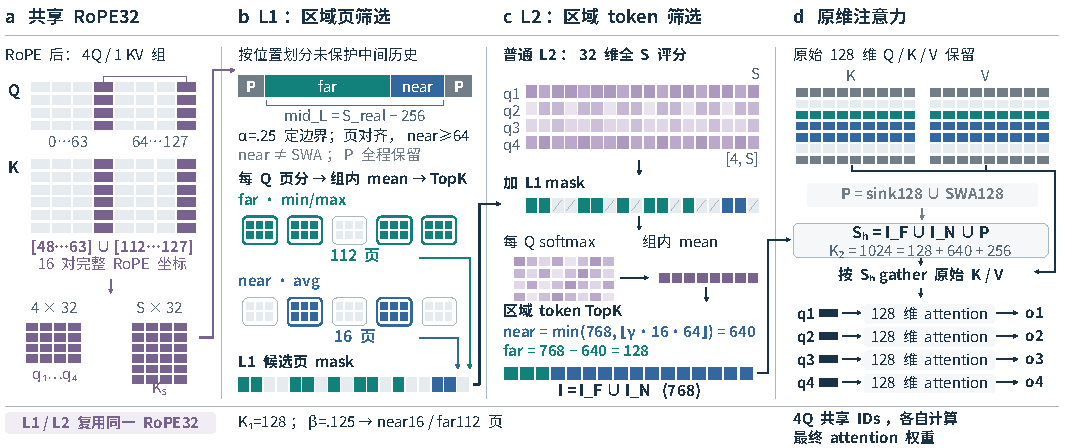
\includegraphics[width=\textwidth]{ppt_near_far_zh.pdf}
\par\medskip\noindent 区域筛选与保护预算。候选充足时，128页配额分成near16／far112页；总1024词元包含256保护与640／128近远词元。图块数量仅示意。逐查询头归一化后才在KV组内平均。
\clearpage
\section*{机制补充图 S3: 从prefill观测到decode复用的gate生命周期}
\noindent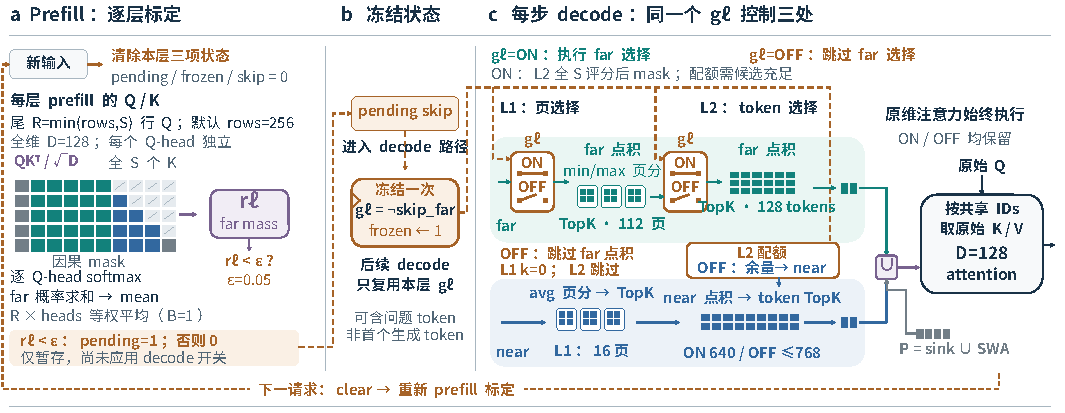
\includegraphics[width=\textwidth]{ppt_gate_zh.pdf}
\par\medskip\noindent Gate生命周期与支持的短路。prefill暂存决定，首次decode路径调用冻结。在有效长度、far非空的固定数值配额路径上，OFF跳过far L1/L2点积与选取，只把L2余量回填near，L1 near仍16页。全域准备、S宽缓冲及softmax成本保留。gate默认关闭，双32主线的匹配质量／成本尚未验证。
\clearpage
\section*{补充图 S4：描述性配置比较}
\noindent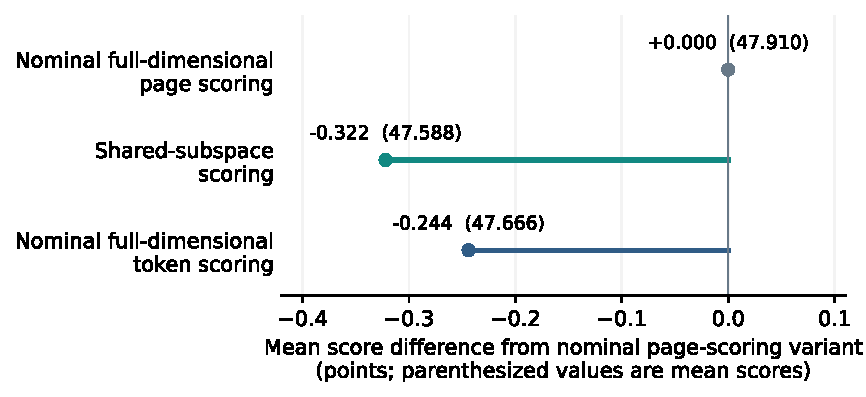
\includegraphics[width=.72\textwidth]{e134_quality_current.pdf}
\par\medskip\noindent 五任务均值为47.910（名义full/sub）、47.588（sub/sub）与47.666（名义sub/full）。相对sub/sub的0.322、0.078分差值仅作描述。Full/sub缺配置旁车，sub/full的L2模式标记未绑定到实现该模式的生产代码树，因此这些标签不能建立受控阶段干预或已完成的三臂消融。补充注S7列出配置证据。这些均不是dense FullKV，也不建立文档配对非劣性或匹配质量--成本结论。
\clearpage
\section*{补充注 S5：Gate观测与执行范围}

功能未启用时仍执行普通far选择；图中OFF仅指启用功能后标定得到的逐层跳过决定。D$'$扩展在每层prefill观测后暂存pending决定，在首次decode路径调用时冻结，后续复用直到新输入清空（补充图S3）。该调用可能仍在消费question token，不能据此假定已经看完整问题。标定使用末尾至多256行可用Q、原维评分及逐Q头softmax，对平均far注意力质量做严格阈值比较；该阈值只用于prefill观测的判定，并不约束后续decode的远区注意力概率质量或任务误差。



在支持的数值配额路径（batch为1、有效长度已知且far非空）中，OFF跳过far L1/L2点积与选取，仅将剩余L2配额回填合法near词元，不扩大near的L1页预算。far-on、off-refill、off-no-refill是不同干预。移除far会改变逐Q softmax分母及组平均near排序，因此回填不是保持near选集不变的单纯省算。准备、量化、repeat-to-float和S宽缓冲／softmax均计入成本。动态与静态skip组合被显式拒绝，Llama动态注册也被拒绝；批内状态隔离、真实生命周期和分布变化回退仍需运行验证。独立的动态$\alpha,\beta,\gamma$求解器继续暂停。


主文gate是双32方法的候选扩展。现有gate任务汇总缺完整子空间配置与配对预测，不能用于验证该配置。上述实现细节限定机制适用范围，并非实测速度或质量收益。

\clearpage
\section*{补充注 S6：历史诊断的适用范围}
以下保留主文限制所依据的详细数值。这些是作者归档诊断，不是新实验，也不是双32方法的匹配验证。

\textbf{选择器局部计时与汇总。}归档性能记录对新实现进行两轮GPU交换测量。每轮值分别为full/sub的1.3635／1.337毫秒、sub/sub的1.3872／1.3324毫秒、sub/full的1.4794／1.4473毫秒。记录给出的两轮中位汇总分别为1.3502、1.3598、1.4634毫秒。对每一对数值在本地取通常的中点中位数，可得1.35025、1.35980、1.46335毫秒，解释了此前额外的小数位；这一算术复算不是新计时。原件未提供逐阶段中位数或原始序列，因此不能确认此前“五阶段中位数之和”的描述。合成单层、batch1、单query、64K的范围不同于完整层或请求，也未与质量作业配对。记录称60步、40次预热及20个稳态样本，但此前检查的harness对应100总步及60个稳态样本；矛盾仍未解决。所报sub/sub时间高于full/sub，既未确立统计显著性，也未建立完整系统加速。

\textbf{区域与gate诊断。}历史保护only均值26.09，含middle检索47.91，但预算也从1024降到256，无法隔离区域策略贡献。Gate标定包含16输入、每个36层；保存far-mass字段$<.05$的输入--层记录在prefill／decode分别30／22条，交集13。prefill选中记录的decode far注意力质量均值0.0582、最大0.1678，表明跨阶段变化，不能证明任务精度保持或请求收益。

后续作者汇总在$\epsilon=.05/.10$时五任务均值47.876／47.692，对复用47.910锚分别下降0.034／0.218分。每臂3项任务下降，HotpotQA下降1.05／1.26分。作者五任务bootstrap区间$[-.584,.452]/[-.806,.400]$仅为描述，跨零不证明等价。现有作业记录尚不能建立双32配置的匹配比较（补充注S5）；三政策质量及完整成本仍未匹配验证。

当前双低频32缺匹配dense FullKV质量参照、稀疏full/full选择器对照及包含准备成本的请求比较。旧full-L1/tail32记录不能改名补齐。128K RULER记录（主文文献[10]）中的新FullKV回执不补齐旧稀疏臂有效配置，无法支持跨臂排名。历史静态逐层表未达到提升门槛，旧quota/gate又混变多种政策或尺度；这些负结果约束解释，但不直接检验当前子空间和prefill gate。原始记录与失败历史保持。


\clearpage
\section*{补充注 S7：预算与配置身份}
\textbf{公平比较。}稀疏对手的预算以最终去重注意力选集$K$对齐，保护词元包含其中。L1候选页属于内部设计，不要求与对手相同；其构造、评分、排序和访存均计入成本。模型、输入ID、生成上限、prefill/decode处理、dense层策略及任务scorer应匹配。原生实现与受控适配器结果分别报告。名义$K$之外，还需报告页取整后的实际词元数与选集共享粒度。

\textbf{Sub/sub LongBench设置。}五份manifest明确页长64、L1上限128页、最终上限1024词元、压缩比4、tail坐标、$\alpha=.25$、$\beta=.125$、$\gamma=.625$、near平均／far minmax页评分及4-bit量化--反量化数值，并明确共享KV头选集、dense prefill、静态跳层关闭。五份运行记录均绑定生产提交\texttt{35b39bd8\allowbreak{}e43cf478\allowbreak{}bb4f0ab6\allowbreak{}4a8457f0\allowbreak{}8d87c864}。该源码给出32维评分、前缀保护$2\times64=128$、近期保护128，以及Qwen3各层稀疏decode。这些源码推断字段不能核实未记录的修改工作树或运行trace。正常长历史路径分配near/far各16/112页、middle各640/128词元，并加入256保护词元。8192个候选槽位不等于最终使用8192个注意力词元，也不约束L2评分量：普通L2仍完整历史评分后mask。逐步实际计数未记录。

保存的输入上限为31500；各任务样本数／最大生成词元数为：Qasper 200/128、HotpotQA 200/32、MuSiQue 200/32、GovReport 200/512、RepoBench-P 500/64。上限不等于实际输入长度。这些配置旁车不能建立完整模型／tokenizer版本、运行精度、硬件身份与scorer版本，匹配比较须另行绑定。非劣检验仍需文档簇身份、匹配dense运行以及事前规定的任务质量容差。

\textbf{名义full/sub。}五份历史预测无manifest或运行回执。文件名／verdict可定位页长64、L1上限128、最终上限1024、压缩比4及相同名义$\alpha,\beta,\gamma$。有效输入上限、完整生产身份、保护、阶段和完整scorer设置未核实，不能用当前默认值补齐。

\textbf{名义sub/full。}五份manifest含上述预算设置及full L2标记。四份回执缺生产提交；MuSiQue记录为\texttt{60027fba\allowbreak{}3672f337\allowbreak{}44917c4f\allowbreak{}59960d0f\allowbreak{}131f8ab0}，但该代码树没有实现记录中的L2模式字段。因此，该提交不能确定实际执行的代码。保留名义标签和得分，不认证实际全维L2执行。

\textbf{Quest对手。}官方评测采用多词元dense prefill、逐词元稀疏处理、前两层dense及逐Q头选页。其1024词元预算与16词元页长，在内部不同于本文128个64词元页。受控比较对齐最终去重$K$与阶段／层策略，页配额和头共享差异单列。论文原生配置与受控适配器不得混合为一个结果。本文不声称已完成匹配Quest或FullKV的质量--请求成本比较。

\textbf{其他结果族。}64K合成选择器计时为单层、batch一、单query汇总，采样协议仍存在矛盾（S6），未与LongBench请求绑定。Gate汇总记录阈值但未明确完整生产／子空间配置。保护only使用256词元，对照使用1024。缺少的身份、未知gate/refill设置及未测完整成本均保持未知，不以当前默认值推断。

\end{document}
